\documentclass[a4paper,12pt]{article}

\newcommand{\solution}[1]{\textcolor{red}{\ifsol\newline#1\fi}}
\newcommand{\comment}[1]{\textcolor{blue}{\emph{Comment: #1}}}

\usepackage{graphicx}
\usepackage{fullpage}
\usepackage{amsmath}
\usepackage{amssymb,amsthm}
\usepackage[totalwidth=166mm,totalheight=240mm]{geometry}
\usepackage{hyperref}
\usepackage{float}
\usepackage{paralist}

% Packages for pseudo-code
\usepackage{algorithm}
\usepackage{algpseudocode}
% Packages for colors
\usepackage{xcolor}
% Package for comments
\usepackage{verbatim}
\usepackage{lscape}

% \parindent0mm
% \pagestyle{empty}


\usepackage{tikz}
\usetikzlibrary{arrows}

\newtheorem{theorem}{Theorem}

\newcounter{aufgc}
\newenvironment{exercise}[2]%
{\noindent\refstepcounter{aufgc}\textbf{Exercise \arabic{aufgc}} \emph{#1} (#2 points)\\}
{

  \noindent\hrulefill\medskip}%

\newtheorem{lemma}[theorem]{Lemma}

\renewcommand{\labelenumi}{(\alph{enumi})}

\newcommand{\sheetnumber}{1}
\newcommand{\id}{192.020}
\newcommand{\semester}{WS 2023/24}
\newcommand{\session}{01.12.2023, 10:00-12:00}
\newcommand{\handin}{28.11.2023}
\newcommand{\room}{FAV EG C}

\newcommand{\authorOne}{Matteo Migliarini 12306959}
\newcommand{\authorTwo}{Nicola Maestri 12306354}
\newcommand{\groupno}{30} %Leave unchanged for first exercise sheet

\begin{document}

% Header
\noindent\hrulefill\medskip
\begin{center}
  {\large \bf TU Wien\ -- \semester\\[1mm]
    Heuristic Optimization Techniques\\[1mm]
    Programming Assigmnent 2}\\[0.5mm]
  \bigskip
  
  {\authorOne\linebreak\authorTwo}
  \medskip\\
  {Group \groupno}
\end{center}
\vspace{0.1cm}
\noindent\hrulefill\medskip

% Report

\section*{Genetic Algorithm for WsPEP}
\begin{algorithm}
\caption{Genetic Algorithm}
\begin{algorithmic}

\State $t \gets generation\ 0$
\State initialize $P(t)$
\State evaluate $P(t)$
\While {not termination condition}
    \State $parent\_1 \gets selection(P(t))$
    \State $parent\_2 \gets selection(P(t))$
    \State $child \gets crossover(parent\_1,parent\_2)$
    \State $child \gets mutation(child)$
    \State $P(t+1) \gets replace(P(t),child)$
    \State $t \gets t+1$
\EndWhile

\noindent
\Return $P(t)$
\end{algorithmic}
\end{algorithm}

\subsection*{Initialization}
The algorithm is implemented as a class and the initialization of the population is performed when the class is instantiated. The population is an attribute of the created object and its length is by default $100$, although it is possible to set this parameter differently.\\
To ensure diversity in the initial population, individuals are created using various random greedy construction methods; in particular:
\begin{itemize}
    \item $75\%$ of individuals are generated by \emph{randomized\_Karger\_construction}\\
    (Nodes are clustered first, followed by the addition of edges to form s-plexes)
    \item $25\%$ of individuals are generated by \emph{reinserting\_greedy\_construction} in a randomized setting.\\
    (we reinsert edges in a random way guaranteeing that clusters are always s-plexes)
    \item $1$ individual is result of a deterministic greedy construction
\end{itemize}

\subsection*{Selection}
At each step two parents are selected among the population and recombined to create a new individual. The new solution is added to the population and then the one with the worst fitness is discarded.\\
The selection can be performed either uniformly at random or through roulette-wheel selection. In our experiments, we opted for a random selection to favor the exploration of the solution space.\\

\subsection*{Crossover}
Given two parents, crossover aims to create a child whose clusters satisfy these two principles:
\begin{itemize}
    \item Nodes connected in both parents are connected in the child
    \item Nodes separated in both parents are separated in the child
\end{itemize}
In our implementation we guarantee only the first claim creating a cluster for each node as intersection of the two parents' clusters which the node belongs to.
This operation results in some clusters being very small, and therefore, there is a need to merge some of them according to some rule. One possible way is to exploit a heuristic which estimates the goodness of the final merged clusters and then decide if to perform or not the operation.\\
We instead opted for another way, two clusters are selected and are merged with a certain probability. The clusters are selected with a probability inversely proportional to their length and merged with a certain probability depending on a parameter alpha. The operation is performed $10$ times in a crossover and small clusters are more likely to be selected for the merging. Parameter alpha ideally controls how much randomness is added to the recombination of the clusters: with $\alpha=0$ a lot of information from parents is kept, whereas $\alpha=1$ means that only a little information is preserved.

\subsection*{Mutation}
The task of crossover is to cluster nodes according to the parents, mutation adds some randomness and tries to improve the quality of the s-plexes.\\
First swap node exchanges nodes in two clusters, then we use a fixed length local search to improve the quality of the s-plexes with neighbourhood \emph{Flip\_Edge}. 

\subsection*{Termination Condition}
The termination conditions are as follows:
\begin{itemize}
    \item $max\ number\ of\ generations\ = 3000$
    \item $600$ consecutive generations without any improvement
\end{itemize}

\begin{figure}[H]
\centering
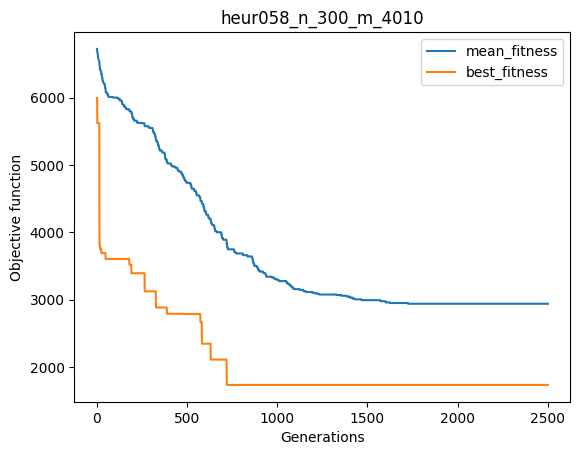
\includegraphics[width=10cm]{graphics/grafico1.png}
\end{figure}

\section*{Genetic Algorithm Tuning}
Parameter $alpha$ controls the probability of merging two selected clusters in the crossover: $alpha=0$ corresponds to never merging them, while $\alpha=1$ corresponds to always merging them.\\
The table below shows results obtained by tuning instances with different settings of $\alpha$.\\
For each instance we report:
\begin{itemize}
    \item mean and best fitness of final population after in 10 different runs
    \item average mean and best fitness achieved by the algorithm
    \item improvement with respect to initial population
\end{itemize}

\noindent
\textbf{Difference between $\alpha=0.0$ and $\alpha=0.5$ is statistically significant}\\
- level of significance: $0.05$\\
- $H_0:=$ "The difference is not significant"\\
- $H_1:=$ "The difference is significant"\\

\noindent
Test Result:\\
p-value = 0.0178\\
$H_0$ can be rejected on a level of significance of 0.05.\\

\noindent
\textbf{Results with $\alpha=0.5$ are greater than ones with $\alpha=0.5$}\\
- level of significance: $0.05$\\
- $H_0:=$ "Results with $\alpha=0.5$ are lower or equl to the ones with $\alpha=0.5$"\\
- $H_1:=$ "Results with $\alpha=0.5$ are greater than ones with $\alpha=0.0$"\\

\noindent
Test Result:\\
p-value = 0.0089\\
$H_0$ can be rejected on a level of significance of 0.05.\\

\noindent
\textbf{Difference between $\alpha=0.0$ and $\alpha=1.0$ is statistically significant}\\
- level of significance: $0.05$\\
- $H_0:=$ "The difference is not significant"\\
- $H_1:=$ "The difference is significant"\\

\noindent
Test Result:\\
p-value = 0.1315\\
$H_0$ cannot be rejected on a level of significance of 0.05.\\

\begin{figure}[H]
\centering
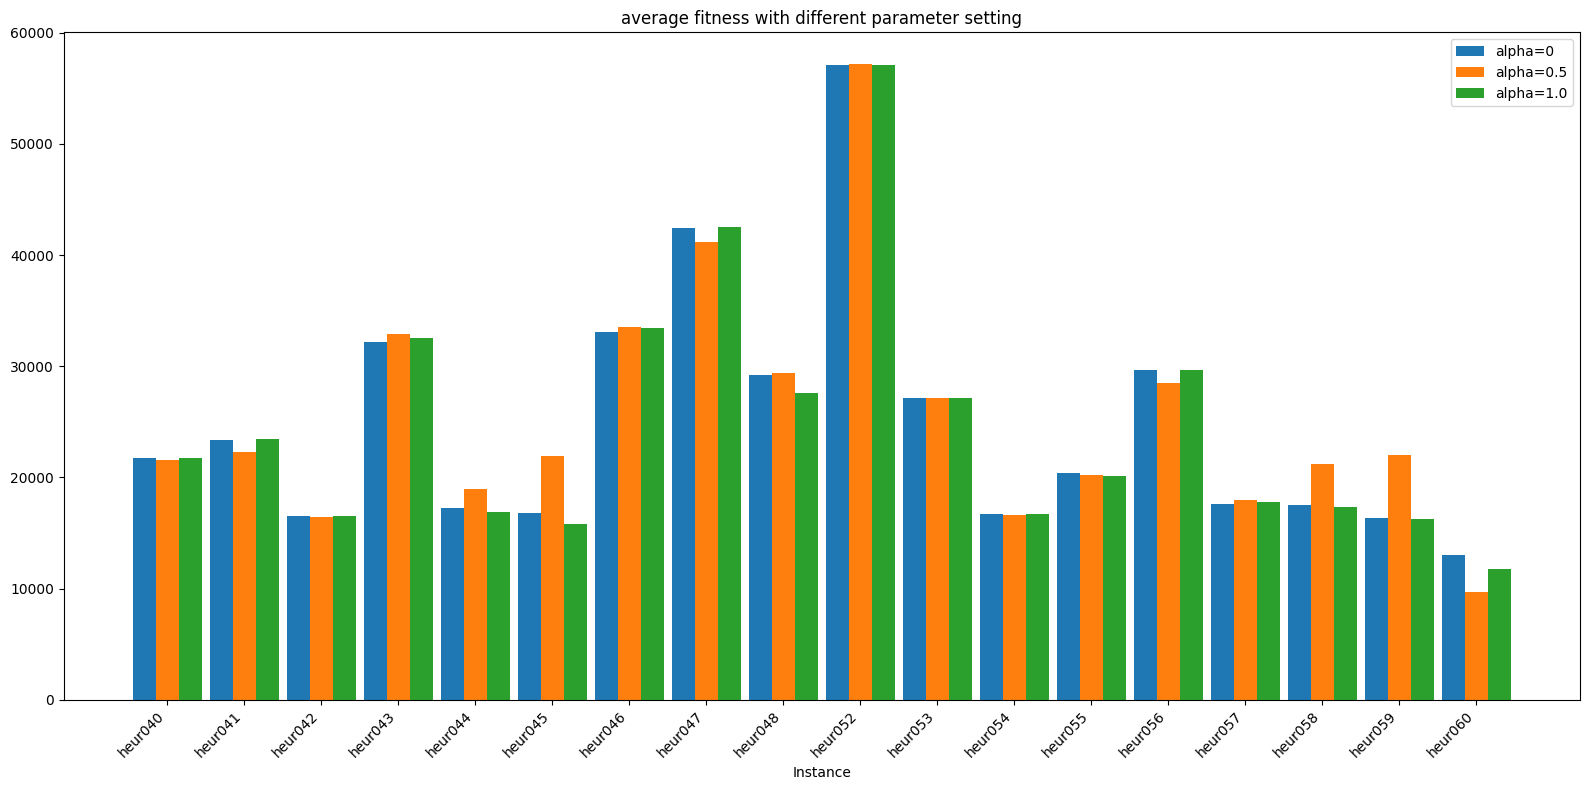
\includegraphics[width=17cm]{graphics/mean 3.png}
\end{figure}

\begin{figure}[H]
\centering
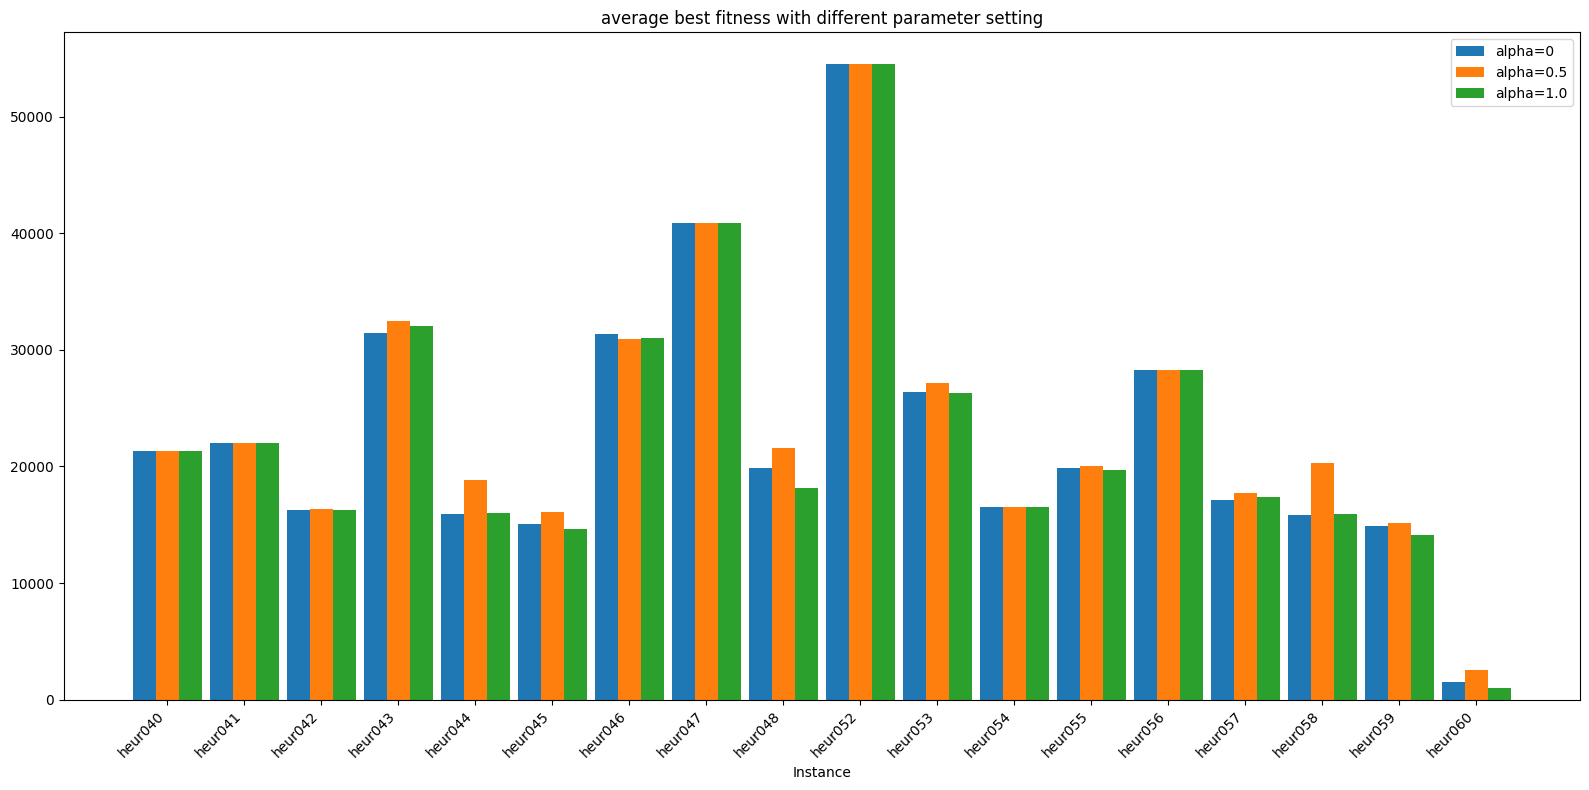
\includegraphics[width=17cm]{graphics/min 2.png}
\end{figure}

\newpage
% \begin{landscape}
\begin{table}[H]
    \centering
    \begin{tabular}{l|c|r|r|r|r|r|r}
        istance  &   & run 1     & run 2  & run 3     & run 4     & run 5      & average \\ %&& run 6     & run 7     & run 8     & run 9     & run 10   improvement\\
        \hline
        heur040 & mean & 6728.56 & 6694.46 & 6736.04 & 6740.42 & 6735.36 & 6745.974 \\ %& NO\\ & 6732.32 & 6797.8 & 6786.72 & 6769.13 & 6738.93 
                & best & 6384    & 6279    & 6361    & 6378    & 6371    & 6365.4   \\ %& \\& 6362    & 6395   & 6363    & 6386    & 6375    
        \hline
        heur041 & mean & 8417.01 & 8206.55 & 8353.46 & 8353.75 & 8445.24  & 8395.596 \\ %& NO\\& 8538.19 & 8366.21& 8445.04 & 8532.88 & 8297.63
                & best & 7039    & 7039    & 7039    & 7039    & 7039     & 7039 \\ %& \\& 7039    & 7039   & 7039    & 7039    & 7039   
        \hline
        heur042 & mean & 1539.89 & 1505.31 & 1517.13 & 1536.74 & 1512.99 & 1518.123  \\%& NO\\& 1498.2  & 1498.37 & 1507.34 & 1529.7 & 1535.56 
                & best & 1323    & 1258    & 1239    & 1278    &   1226   & 1242.7 \\ %& \\& 1256    & 1197    & 1167    & 1244   & 1239   
        \hline
        heur043 & mean & 16933.81& 17563.57& 16992.52& 17190.13& 17312.08 & 17150.35 \\%& YES \\& 16244.59& 17270.28& 16161.45& 18410.35& 17424.73
                & best & 16327   & 17125   & 16725   & 16858   & 16994   & 16423.7 \\%& \\& 14996   & 16762   & 14867   & 16437   & 17146   
        \hline
        heur044 & mean & 2405.09 & 2333.69 & 1870.92 & 2647.45 & 2146.68 & 2280.766 \\%& YES\\& & & & & 
                & best & 564     & 627     & 1264    & 939     & 1272    & 933.2 \\ %& \\&  & & & & & 933.2 \\ %& \\
        \hline
        heur045 & mean & 2137.4 & 941.68  & 2106.51 & 2282.71 & 1555.62 & 1804.784 \\%& YES\\& & & & & 
                & best & 154    & 212     & 442     & -34     & -369    & 81.0 \\ %& \\ &  & & & &
        \hline
        heur046 & mean & 18839.56 & 17331.27 & 18957.86 & 17096.66 & 18090.42 & 18063.154 \\%& YES\\& & & & & 
                & best & 16825    & 15564    & 17496    & 15628    & 16092    & 16321.0 \\ %& \\&  & & & & 
        \hline
        heur047 & mean & 27496.3  & 27397.13 & 27573.2  & 27504.37 & 27382.75 & 27470.75\\%& YES\\& & & & & 
                & best & 25893    & 25905    & 25879    & 25901    & 25910    &  25897.6 \\ %& \\&  & & & & 
        \hline
        heur048 & mean & 14135.35 & 14287.07 & 14280.42 & 13026.6  & 15223.64 & 14190.616\\%& YES\\& & & & & 
                & best & 6743     &  3169    & 4559     & 4266     & 5720     &  4891.4 \\ %& \\&  & & & & 
        \hline
        heur052 & mean & 42271.24 & 41967.6 & 42052.98 & 41983.49 & 42027.17 & 42060.496 \\
                & best & 39500 & 39522 & 39444 & 39444 & 39588 & 39499.6 \\
        \hline
        heur053 & mean & 12155.9 & 12141.08 & 12129.29 & 12144.05 & 12150.61 & 12144.186\\
                & best & 11589 & 11217 & 11222 & 11422 & 11278 & 11345.6\\
        \hline
        heur054 & mean & 1715.32 & 1714.04 & 1720.21 & 1703.05 & 1707.6 & 1712.04 \\
                & best & 1563 & 1573 & 1572 & 1574 & 1548 & 1566.0 \\
        \hline
        heur055 & mean & 5562.2 & 4731.02 & 5559.22 & 5407.2 & 5614.7 & 5374.868 \\
                & best & 5005 & 4417 & 4991 & 5046 & 5023 & 4896.4\\
        \hline
        heur056 & mean & 14670.74 & 14722.92 & 14623.08 & 14677.68 & 14559.82 & 14650.848 \\
                & best & 13240 & 13237 & 13242 & 13240 & 13238 & 13239.4 \\
        \hline
        heur057 & mean & 2680.81 & 2775.21 & 2375.06 & 2663.67 & 2641.77 & 2627.304 \\
                & best & 2217 & 1860 & 2011 & 2301 & 2198 & 2117.4\\
        \hline
        heur058 & mean & 2518.19 & 2667.96 & 2028.02 & 2228.38 & 3023.32 & 2493.174\\
                & best & 1054 & 649 & 772 & 73  & 1819  & 873.4\\
        \hline
        heur059 & mean & 1343.89 & 1627.86 & 1012.8 & 927.62 & 1697.48 &  1321.93 \\
                & best & -56 & 504 & -685 & 0 & -146 & -76.6\\
        \hline
        heur060 & mean & -1149.66 & -2188.28 & -2646.34 & -1231.64 & -2892.24 & -2021.632 \\
                & best & -13602 & -13714 & -12518 & -13718 & -13833 & -13477.0 \\
    \end{tabular}
    \caption{$\alpha = 0.0$}
    \label{tab:my_label}
\end{table} 
% \end{landscape}
\noindent
\emph{Note:} the reported fitness may appears negative in the table because is not scaled.\\ To encourage insertion of already present edges their weights are set negative, however we forgot to scale the results in the fitness function and there was no time to run all instances again. The minimum can therefore be negative but this should not be an issue when we compare results obtained with different parameter settings cause we focus on the difference of the two performances.


\begin{comment}
heur040\_n\_300\_m\_13358
Improvement: NO
Best fitness: 6365.4
[6384, 6279, 6361, 6378, 6371, 6362, 6395, 6363, 6386, 6375]
Mean fitness: 6745.973999999999
[6728.56, 6694.46, 6736.04, 6740.42, 6735.36, 6732.32, 6797.8, 6786.72, 6769.13, 6738.93]

heur041_n_300_m_17492.txt
Best fitness: 7039.0
[7039, 7039, 7039, 7039, 7039, 7039, 7039, 7039, 7039, 7039]
Mean fitness: 8395.596000000001
[8417.01, 8206.55, 8353.46, 8353.75, 8445.24, 8538.19, 8366.21, 8445.04, 8532.88, 8297.63]

heur042_n_300_m_5764.txt
Best fitness: 1242.7
[1323, 1258, 1239, 1278, 1226, 1256, 1197, 1167, 1244, 1239]
Mean fitness: 1518.123
[1539.89, 1505.31, 1517.13, 1536.74, 1512.99, 1498.2, 1498.37, 1507.34, 1529.7, 1535.56]
heur043_n_300_m_12914.txt

heur043_n_300_m_12914.txt
Improvement: YES
Best fitness: 16423.7
[16327, 17125, 16725, 16858, 16994, 14996, 16762, 14867, 16437, 17146]
Mean fitness: 17150.351000000002
[16933.81, 17563.57, 16992.52, 17190.13, 17312.08, 16244.59, 17270.28, 16161.45, 18410.35, 17424.73]

heur044_n_300_m_3234.txt
Best fitness: 933.2
[564, 627, 1264, 939, 1272]
Mean fitness: 2280.7660000000005
[2405.09, 2333.69, 1870.92, 2647.45, 2146.68]

heur045_n_300_m_6293.txt
Improvement: YES
Best fitness: 81.0
[154, 212, 442, -34, -369]
Mean fitness: 1804.784
[2137.4, 941.68, 2106.51, 2282.71, 1555.62]

heur046_n_300_m_13150.txt
Improvement: YES
Best fitness: 16321.0
[16825, 15564, 17496, 15628, 16092]
Mean fitness: 18063.154000000002
[18839.56, 17331.27, 18957.86, 17096.66, 18090.42]

heur047_n_300_m_20096.txt
Best fitness: 25910
Best fitness: 25897.6
[25893, 25905, 25879, 25901, 25910]
Mean fitness: 27470.75
[27496.3, 27397.13, 27573.2, 27504.37, 27382.75]

heur048_n_300_m_14666.txt
Best fitness: 4891.4
[6743, 3169, 4559, 4266, 5720]
Mean fitness: 14190.615999999998
[14135.35, 14287.07, 14280.42, 13026.6, 15223.64]
\end{comment}

\begin{comment}
heur040\_n\_300\_m\_13358
Generation 0
Mean fitness: 6728.56
Best fitness: 6384
Generation 1000
Mean fitness: 6728.56
Best fitness: 6384
Generation 2000
Mean fitness: 6728.56
Best fitness: 6384
Generation 0
Mean fitness: 6694.46
Best fitness: 6279
Generation 1000
Mean fitness: 6694.46
Best fitness: 6279
Generation 2000
Mean fitness: 6694.46
Best fitness: 6279
Generation 0
Mean fitness: 6736.04
Best fitness: 6361
Generation 1000
Mean fitness: 6736.04
Best fitness: 6361
Generation 2000
Mean fitness: 6736.04
Best fitness: 6361
Generation 0
Mean fitness: 6740.42
Best fitness: 6378
Generation 1000
Mean fitness: 6740.42
Best fitness: 6378
Generation 2000
Mean fitness: 6740.42
Best fitness: 6378
Generation 0
Mean fitness: 6735.36
Best fitness: 6371
Generation 1000
Mean fitness: 6735.36
Best fitness: 6371
Generation 2000
Mean fitness: 6735.36
Best fitness: 6371
Generation 0
Mean fitness: 6732.32
Best fitness: 6362
Generation 1000
Mean fitness: 6732.32
Best fitness: 6362
Generation 2000
Mean fitness: 6732.32
Best fitness: 6362
Generation 0
Mean fitness: 6797.8
Best fitness: 6395
Generation 1000
Mean fitness: 6797.8
Best fitness: 6395
Generation 2000
Mean fitness: 6797.8
Best fitness: 6395
Generation 0
Mean fitness: 6786.72
Best fitness: 6363
Generation 1000
Mean fitness: 6786.72
Best fitness: 6363
Generation 2000
Mean fitness: 6786.72
Best fitness: 6363
Generation 0
Mean fitness: 6769.13
Best fitness: 6386
Generation 1000
Mean fitness: 6769.13
Best fitness: 6386
Generation 2000
Mean fitness: 6769.13
Best fitness: 6386
Generation 0
Mean fitness: 6738.93
Best fitness: 6375
Generation 1000
Mean fitness: 6738.93
Best fitness: 6375
Generation 2000
Mean fitness: 6738.93
Best fitness: 6375
Best fitness: 6365.4
[6384, 6279, 6361, 6378, 6371, 6362, 6395, 6363, 6386, 6375]
Mean fitness: 6745.973999999999
[6728.56, 6694.46, 6736.04, 6740.42, 6735.36, 6732.32, 6797.8, 6786.72, 6769.13, 6738.93]

heur041_n_300_m_17492.txt
Generation 0
Mean fitness: 8417.01
Best fitness: 7039
Generation 1000
Mean fitness: 8417.01
Best fitness: 7039
Generation 2000
Mean fitness: 8417.01
Best fitness: 7039
Generation 0
Mean fitness: 8206.55
Best fitness: 7039
Generation 1000
Mean fitness: 8206.55
Best fitness: 7039
Generation 2000
Mean fitness: 8206.55
Best fitness: 7039
Generation 0
Mean fitness: 8353.46
Best fitness: 7039
Generation 1000
Mean fitness: 8353.46
Best fitness: 7039
Generation 2000
Mean fitness: 8353.46
Best fitness: 7039
Generation 0
Mean fitness: 8353.75
Best fitness: 7039
Generation 1000
Mean fitness: 8353.75
Best fitness: 7039
Generation 2000
Mean fitness: 8353.75
Best fitness: 7039
Generation 0
Mean fitness: 8445.24
Best fitness: 7039
Generation 1000
Mean fitness: 8445.24
Best fitness: 7039
Generation 2000
Mean fitness: 8445.24
Best fitness: 7039
Generation 0
Mean fitness: 8538.19
Best fitness: 7039
Generation 1000
Mean fitness: 8538.19
Best fitness: 7039
Generation 2000
Mean fitness: 8538.19
Best fitness: 7039
Generation 0
Mean fitness: 8366.21
Best fitness: 7039
Generation 1000
Mean fitness: 8366.21
Best fitness: 7039
Generation 2000
Mean fitness: 8366.21
Best fitness: 7039
Generation 0
Mean fitness: 8445.04
Best fitness: 7039
Generation 1000
Mean fitness: 8445.04
Best fitness: 7039
Generation 2000
Mean fitness: 8445.04
Best fitness: 7039
Generation 0
Mean fitness: 8532.88
Best fitness: 7039
Generation 1000
Mean fitness: 8532.88
Best fitness: 7039
Generation 2000
Mean fitness: 8532.88
Best fitness: 7039
Generation 0
Mean fitness: 8297.63
Best fitness: 7039
Generation 1000
Mean fitness: 8297.63
Best fitness: 7039
Generation 2000
Mean fitness: 8297.63
Best fitness: 7039
Best fitness: 7039.0
[7039, 7039, 7039, 7039, 7039, 7039, 7039, 7039, 7039, 7039]
Mean fitness: 8395.596000000001
[8417.01, 8206.55, 8353.46, 8353.75, 8445.24, 8538.19, 8366.21, 8445.04, 8532.88, 8297.63]

heur042_n_300_m_5764.txt
Generation 0
Mean fitness: 1539.89
Best fitness: 1323
Generation 1000
Mean fitness: 1539.89
Best fitness: 1323
Generation 2000
Mean fitness: 1539.89
Best fitness: 1323
Generation 0
Mean fitness: 1505.31
Best fitness: 1258
Generation 1000
Mean fitness: 1505.31
Best fitness: 1258
Generation 2000
Mean fitness: 1505.31
Best fitness: 1258
Generation 0
Mean fitness: 1517.13
Best fitness: 1239
Generation 1000
Mean fitness: 1517.13
Best fitness: 1239
Generation 2000
Mean fitness: 1517.13
Best fitness: 1239
Generation 0
Mean fitness: 1536.74
Best fitness: 1278
Generation 1000
Mean fitness: 1536.74
Best fitness: 1278
Generation 2000
Mean fitness: 1536.74
Best fitness: 1278
Generation 0
Mean fitness: 1512.99
Best fitness: 1226
Generation 1000
Mean fitness: 1512.99
Best fitness: 1226
Generation 2000
Mean fitness: 1512.99
Best fitness: 1226
Generation 0
Mean fitness: 1498.2
Best fitness: 1256
Generation 1000
Mean fitness: 1498.2
Best fitness: 1256
Generation 2000
Mean fitness: 1498.2
Best fitness: 1256
Generation 0
Mean fitness: 1498.37
Best fitness: 1197
Generation 1000
Mean fitness: 1498.37
Best fitness: 1197
Generation 2000
Mean fitness: 1498.37
Best fitness: 1197
Generation 0
Mean fitness: 1507.34
Best fitness: 1167
Generation 1000
Mean fitness: 1507.34
Best fitness: 1167
Generation 2000
Mean fitness: 1507.34
Best fitness: 1167
Generation 0
Mean fitness: 1529.7
Best fitness: 1244
Generation 1000
Mean fitness: 1529.7
Best fitness: 1244
Generation 2000
Mean fitness: 1529.7
Best fitness: 1244
Generation 0
Mean fitness: 1535.56
Best fitness: 1239
Generation 1000
Mean fitness: 1535.56
Best fitness: 1239
Generation 2000
Mean fitness: 1535.56
Best fitness: 1239
Best fitness: 1242.7
[1323, 1258, 1239, 1278, 1226, 1256, 1197, 1167, 1244, 1239]
Mean fitness: 1518.123
[1539.89, 1505.31, 1517.13, 1536.74, 1512.99, 1498.2, 1498.37, 1507.34, 1529.7, 1535.56]
heur043_n_300_m_12914.txt

heur043_n_300_m_12914.txt
Generation 0
Mean fitness: 18867.4
Best fitness: 17441
Generation 1000
Mean fitness: 16946.24
Best fitness: 16327
Generation 2000
Mean fitness: 16933.81
Best fitness: 16327
Generation 0
Mean fitness: 18915.95
Best fitness: 17447
Generation 1000
Mean fitness: 18132.92
Best fitness: 17447
Generation 2000
Mean fitness: 17728.17
Best fitness: 17447
Generation 0
Mean fitness: 18823.94
Best fitness: 17415
Generation 1000
Mean fitness: 17119.41
Best fitness: 16725
Generation 2000
Mean fitness: 17010.96
Best fitness: 16725
Generation 0
Mean fitness: 18838.98
Best fitness: 17482
Generation 1000
Mean fitness: 17368.74
Best fitness: 16858
Generation 2000
Mean fitness: 17190.13
Best fitness: 16858
Generation 0
Mean fitness: 18890.79
Best fitness: 17420
Generation 1000
Mean fitness: 17727.43
Best fitness: 17420
Generation 2000
Mean fitness: 17324.21
Best fitness: 16994
Generation 0
Mean fitness: 18856.12
Best fitness: 17475
Generation 1000
Mean fitness: 16474.99
Best fitness: 15204
Generation 2000
Mean fitness: 16244.59
Best fitness: 14996
Generation 0
Mean fitness: 18794.99
Best fitness: 17438
Generation 1000
Mean fitness: 17818.82
Best fitness: 17438
Generation 2000
Mean fitness: 17384.13
Best fitness: 16762
Generation 0
Mean fitness: 19054.82
Best fitness: 17469
Generation 1000
Mean fitness: 18354.68
Best fitness: 15982
Generation 2000
Mean fitness: 16161.45
Best fitness: 14867
Generation 0
Mean fitness: 18940.01
Best fitness: 17460
Generation 1000
Mean fitness: 18940.01
Best fitness: 17460
Generation 2000
Mean fitness: 18940.01
Best fitness: 17460
Generation 0
Mean fitness: 18842.39
Best fitness: 17475
Generation 1000
Mean fitness: 18347.58
Best fitness: 17475
Generation 2000
Mean fitness: 17650.32
Best fitness: 17159
Best fitness: 16423.7
[16327, 17125, 16725, 16858, 16994, 14996, 16762, 14867, 16437, 17146]
Mean fitness: 17150.351000000002
[16933.81, 17563.57, 16992.52, 17190.13, 17312.08, 16244.59, 17270.28, 16161.45, 18410.35, 17424.73]

heur044_n_300_m_3234.txt
Generation 0
Mean fitness: 4427.63
Best fitness: 3880
Generation 1000
Mean fitness: 2405.09
Best fitness: 564
Generation 2000
Mean fitness: 2405.09
Best fitness: 564
Generation 0
Mean fitness: 4378.61
Best fitness: 3880
Generation 1000
Mean fitness: 2448.89
Best fitness: 627
Generation 2000
Mean fitness: 2333.69
Best fitness: 627
Attention: There's an Error!!!
Generation 0
Mean fitness: 4411.94
Best fitness: 3883
Generation 1000
Mean fitness: 1978.51
Best fitness: 1264
Generation 2000
Mean fitness: 1889.96
Best fitness: 1264
Generation 0
Mean fitness: 4393.17
Best fitness: 3878
Generation 1000
Mean fitness: 2782.74
Best fitness: 939
Generation 2000
Mean fitness: 2647.45
Best fitness: 939
Generation 0
Mean fitness: 4339.39
Best fitness: 3879
Generation 1000
Mean fitness: 2367.88
Best fitness: 1458
Generation 2000
Mean fitness: 2174.99
Best fitness: 1272
Best fitness: 933.2
[564, 627, 1264, 939, 1272]
Mean fitness: 2280.7660000000005
[2405.09, 2333.69, 1870.92, 2647.45, 2146.68]

heur045_n_300_m_6293.txt
Generation 0
Mean fitness: 10530.57
Best fitness: 5255
Generation 1000
Mean fitness: 2745.99
Best fitness: 317
Generation 2000
Mean fitness: 2356.79
Best fitness: 317
Attention: There's an Error!!!
Generation 0
Mean fitness: 10604.15
Best fitness: 9166
Generation 1000
Mean fitness: 2148.04
Best fitness: 334
Generation 2000
Mean fitness: 1188.98
Best fitness: 212
Generation 0
Mean fitness: 10475.0
Best fitness: 9156
Generation 1000
Mean fitness: 2265.33
Best fitness: 442
Generation 2000
Mean fitness: 2106.51
Best fitness: 442
Attention: There's an Error!!!
Generation 0
Mean fitness: 10640.64
Best fitness: 9178
Generation 1000
Mean fitness: 2883.19
Best fitness: -34
Generation 2000
Mean fitness: 2616.18
Best fitness: -34
Attention: There's an Error!!!
Generation 0
Mean fitness: 10556.58
Best fitness: 9229
Generation 1000
Mean fitness: 2683.3
Best fitness: -369
Generation 2000
Mean fitness: 1913.15
Best fitness: -369
Attention: There's an Error!!!
Best fitness: 81.0
[154, 212, 442, -34, -369]
Mean fitness: 1804.784
[2137.4, 941.68, 2106.51, 2282.71, 1555.62]

heur046_n_300_m_13150.txt
Generation 0
Mean fitness: 22018.25
Best fitness: 20197
Generation 1000
Mean fitness: 19096.82
Best fitness: 16836
Generation 2000
Mean fitness: 18839.56
Best fitness: 16825
Generation 0
Mean fitness: 21996.33
Best fitness: 20194
Generation 1000
Mean fitness: 17331.27
Best fitness: 15564
Generation 2000
Mean fitness: 17331.27
Best fitness: 15564
Generation 0
Mean fitness: 22135.86
Best fitness: 20157
Generation 1000
Mean fitness: 19047.34
Best fitness: 17496
Generation 2000
Mean fitness: 18957.86
Best fitness: 17496
Generation 0
Mean fitness: 22090.64
Best fitness: 20196
Generation 1000
Mean fitness: 17146.8
Best fitness: 15628
Generation 2000
Mean fitness: 17096.66
Best fitness: 15628
Generation 0
Mean fitness: 21987.24
Best fitness: 20211
Generation 1000
Mean fitness: 18090.42
Best fitness: 16092
Generation 2000
Mean fitness: 18090.42
Best fitness: 16092
Best fitness: 16321.0
[16825, 15564, 17496, 15628, 16092]
Mean fitness: 18063.154000000002
[18839.56, 17331.27, 18957.86, 17096.66, 18090.42]
\end{comment}


% \begin{landscape}
\begin{table}[H]
    \centering
    \begin{tabular}{l|c|r|r|r|r|r|r}
        istance  &   & run 1     & run 2  & run 3     & run 4     & run 5  & average \\ %& improvement\\
        \hline
        heur040 & mean & 6614.04 & 6611.25 & 6607.81 & 6610.21 & 6609.48 & 6610.558\\
                & best & 6358 & 6369 & 6358 & 6364 & 6395 & 6368.8 \\
        \hline
        heur041 & mean & 7264.96 & 7326.48 & 7279.5 & 7274.61 & 7265.68  & 7282.256 \\
                & best & 7039    & 7039    & 7039    & 7039    & 7039    & 7039.0  \\
        \hline
        heur042 & mean & 1474.97 & 1449.84 & 1465.32 & 1468.31 & 1462.38 & 1464.164 \\
                & best & 1379 & 1386 & 1362 & 1388 & 1384  & 1379.8 \\
        \hline
        heur043 & mean & 17871.42 & 17898.28 & 17916.37 & 17846.77 & 18054.6  & 17917.488 \\
                & best & 17453 & 17437 & 17417 & 17421 & 17463 &  17438.2 \\
        \hline
        heur044 & mean & 4004.41 & 3992.71 & 4006.42 & 3984.87 & 4009.16 & 3999.514\\
                & best & 3882 & 3876 & 3879 & 3879 & 3868 & 3876.8 \\
        \hline
        heur045 & mean & 7606.31 & 4522.44 & 7195.58 & 7576.24 & 7951.74 & 6970.462\\
                & best & 1699 & 1205 & 1314 & 555 & 522 & 1059.0\\
        \hline
        heur046 & mean & 18750.47 & 18240.46 & 17754.42 & 18990.14 & 18712.85 & 18489.668 \\
                & best & 16675 & 14494 & 16204 & 16832 & 15248 & 15890.6 \\
        \hline
        heur047 & mean & 26267.45 & 26206.66 & 26123.7 & 26182.95 & 26163.69 & 26188.89\\
                & best & 25901 & 25901 & 25893 & 25901 & 25899 & 25899.0 \\
        \hline
        heur048 & mean & 14442.85 & 14111.43 & 14965.64 & 14487.3 & 13931.26 & 14387.696 \\
                & best & 6727 & 7270 & 8251 & 4979 & 5532 & 6551.8\\
        \hline
        heur052 & mean & 42146.91 & 42231.79 & 42146.04 & 42150.05 & 42246.59 & 42184.276 \\
                & best & 39407 & 39585 & 39496 & 39444 & 39586 & 39503.6 \\
        \hline
        heur053 & mean & 12165.97 & 12170.19 & 12163.47 & 12169.53 & 12184.22 & 12170.676 \\
                & best & 12162 & 12162 & 12162 & 12162 & 12162 & 12162.0\\
        \hline
        heur054 & mean & 1642.64 & 1647.19 & 1648.56 & 1652.11 & 1649.25 & 1647.95 \\
                & best & 1559 & 1556 & 1555 & 1555 & 1576 & 1560.2\\
        \hline
        heur055 & mean & 5196.07 & 5218.11 & 5220.33 & 5201.86 & 5189.1 & 5205.094 \\
                & best & 5038 & 5049 & 5006 & 4999 & 5001 & 5018.6\\
        \hline
        heur056 & mean & 13509.7 & 13498.08 & 13515.82 & 13450.31 & 13425.06 & 13479.794 \\
                & best & 13238 & 13240 & 13240 & 13238 & 13240 & 13239.2\\
        \hline
        heur057 & mean & 2931.65 & 2925.49 & 2874.4 & 2963.3 & 2948.4 & 2928.648\\
                & best & 2702 & 2665 & 2650 & 2794 & 2820 & 2726.2\\
        \hline
        heur058 & mean & 6189.15 & 6163.29 & 6175.37 & 6171.86 & 6189.94 & 6177.922\\
                & best & 5988 & 4680 & 5542 & 4478 & 5987 & 5335.0\\
        \hline
        heur059 & mean & 9121.68 & 9576.07 & 9323.38 & 2621.43 & 4623.5 & 7053.211\\
                & best & -458 & 297 & -717 & 759 & 929 & 162.0\\
        \hline
        heur060 & mean & -4166.99 & -5791.13 & -7729.5 & -2950.81 & -5766.2 & -5280.926\\
                & best & -12103 & -12734 & -12462 & -12139 & -12637 & -12415.0\\

    \end{tabular}
    \caption{$\alpha = 0.5$}
    \label{tab:my_label}
\end{table}
% \end{landscape}

\begin{comment}

heur040_n_300_m_13358.txt
Best fitness: 6368.8
[6358, 6369, 6358, 6364, 6395]
Mean fitness: 6610.558
[6614.04, 6611.25, 6607.81, 6610.21, 6609.48]

heur041_n_300_m_17492.txt
Best fitness: 7039.0
[7039, 7039, 7039, 7039, 7039]
Mean fitness: 7282.255999999999
[7264.96, 7326.48, 7279.55, 7274.61, 7265.68]

heur042_n_300_m_5764.txt
Best fitness: 1379.8
[1379, 1386, 1362, 1388, 1384]
Mean fitness: 1464.1640000000002
[1474.97, 1449.84, 1465.32, 1468.31, 1462.38]

heur043_n_300_m_12914.txt
Best fitness: 17438.2
[17453, 17437, 17417, 17421, 17463]
Mean fitness: 17917.488
[17871.42, 17898.28, 17916.37, 17846.77, 18054.6]

heur044_n_300_m_3234.txt
Best fitness: 3876.8
[3882, 3876, 3879, 3879, 3868]
Mean fitness: 3999.514
[4004.41, 3992.71, 4006.42, 3984.87, 4009.16]

heur045_n_300_m_6293.txt
Best fitness: 1059.0
[1699, 1205, 1314, 555, 522]
Mean fitness: 6970.4619999999995
[7606.31, 4522.44, 7195.58, 7576.24, 7951.74]

heur047_n_300_m_20096.txt
Best fitness: 25899.0
[25901, 25901, 25893, 25901, 25899]
Mean fitness: 26188.89
[26267.45, 26206.66, 26123.7, 26182.95, 26163.69]

heur048_n_300_m_14666.txt
Best fitness: 6551.8
[6727, 7270, 8251, 4979, 5532]
Mean fitness: 14387.696
[14442.85, 14111.43, 14965.64, 14487.3, 13931.26]

heur053_n_300_m_39861.txt
Best fitness: 12162.0
[12162, 12162, 12162, 12162, 12162]
Mean fitness: 12170.676
[12165.97, 12170.19, 12163.47, 12169.53, 12184.22]

heur055_n_300_m_5164.txt
Best fitness: 5018.6
[5038, 5049, 5006, 4999, 5001]
Mean fitness: 5205.094
[5196.07, 5218.11, 5220.33, 5201.86, 5189.1]

heur056_n_300_m_12131.txt
Best fitness: 13239.2
[13238, 13240, 13240, 13238, 13240]
Mean fitness: 13479.794
[13509.7, 13498.08, 13515.82, 13450.31, 13425.06]

heur057_n_300_m_2109.txt
Best fitness: 2726.2
[2702, 2665, 2650, 2794, 2820]
Mean fitness: 2928.648
[2931.65, 2925.49, 2874.4, 2963.3, 2948.4]

heur058_n_300_m_4010.txt
Best fitness: 5335.0
[5988, 4680, 5542, 4478, 5987]
Mean fitness: 6177.922
[6189.15, 6163.29, 6175.37, 6171.86, 6189.94]

heur059_n_300_m_7867.txt
Best fitness: 162.0
[-458, 297, -717, 759, 929]
Mean fitness: 7053.2119999999995
[9121.68, 9576.07, 9323.38, 2621.43, 4623.5]

heur060_n_300_m_12405.txt
Best fitness: -12415.0
[-12103, -12734, -12462, -12139, -12637]
Mean fitness: -5280.926
[-4166.99, -5791.13, -7729.5, -2950.81, -5766.2]


heur054_n_300_m_2746.txt
Generation 0
Mean fitness: 1642.64
Best fitness: 1559
Generation 500
Mean fitness: 1642.64
Best fitness: 1559
Generation 0
Mean fitness: 1647.19
Best fitness: 1556
^[[B^[[B^[[B^[[BGeneration 500
Mean fitness: 1647.19
Best fitness: 1556
Generation 0
Mean fitness: 1648.56
Best fitness: 1555
Generation 500
Mean fitness: 1648.56
Best fitness: 1555
Generation 0
Mean fitness: 1652.11
Best fitness: 1555
Generation 500
Mean fitness: 1652.11
Best fitness: 1555
Generation 0
Mean fitness: 1649.25
Best fitness: 1576
Generation 500
Mean fitness: 1649.25
Best fitness: 1576
Best fitness: 1560.2
[1559, 1556, 1555, 1555, 1576]
Mean fitness: 1647.95
[1642.64, 1647.19, 1648.56, 1652.11, 1649.25]
\end{comment}



% \begin{landscape}
\begin{table}[H]
    \centering
    \begin{tabular}{l|c|r|r|r|r|r|r}
        istance  &   & run 1     & run 2  & run 3     & run 4     & run 5  & average \\ %& improvement\\
        \hline
        heur040 & mean & 6785.91 & 6754.69 & 6730.94 & 6712.12 & 6751.33 & 6746.998 \\
                & best & 6405    & 6398    & 6206    & 6390    & 6361    & 6352.0 \\
        \hline
        heur041 & mean & 8489.1  & 8415.52 & 8415.39 & 8352.28 & 8474.46 & 8429.35 \\
                & best & 7039    & 7039    & 7039    & 7039    & 7039    & 7039.0  \\
        \hline
        heur042 & mean & 1528.2  & 1494.83 & 1523.06 & 1523.52 & 1520.44 & 1518.01 \\
                & best & 1256    & 1218    & 1255    & 1280    & 1214    & 1244.6 \\
        \hline
        heur043 & mean & 17346.17 & 16651.81 & 17329.49 & 17417.41 & 18895.17 & 17528.01 \\
                & best & 17315    & 15807    & 17262    & 17312    & 17431    & 17025.4 \\
        \hline
        heur044 & mean & 3249.38  & 1714.0   & 1084.64  & 1456.41  & 2012.1   & 1903.306 \\
                & best & 2513     & 663      & 167      & 541      & 1081     & 993.0 \\
        \hline
        heur045 & mean & 494.19   & 750.5    & 1256.66  & 595.88   & 827.19 & 784.884\\
                & best & -893     & -630     & 97 & -361     & 53 & -346.8\\
        \hline
        heur046 & mean & 18884.72 & 19866.44 & 17852.56 & 19354.47 & 16460.46 & 18483.73 \\
                & best & 16995    & 19057    & 15668    & 15621    & 12564    & 15981.0 \\
        \hline
        heur047 & mean & 27564.9  & 27515.34 & 27613.38 & 27403.61 & 27462.98 & 27512.042 \\
                & best & 25894    & 25901    & 25920    & 25896    & 25898    & 25901.8\\
        \hline
        heur048 & mean & 13020.54 & 12043.05 & 11952.52 & 13137.55 & 12989.61 & 12628.654 \\
                & best & 4701     & 890      & 3010     & 3472     & 3859     & 3186.4 \\
        \hline
        heur052 & mean & 41985.35 & 42158.81 & 42126.85 & 42039.56 & 42053.09 & 42072.732 \\
                & best & 39444 & 39433 & 39586 & 39500 & 39544 & 39501.4 \\
        \hline
        heur053 & mean & 12172.78 &  12153.45 & 12127.43 & 12147.7 & 12157.99 & 12151.87 \\
                & best & 11407 & 11435 & 11213 & 11181 & 11457 & 11338.6\\
        \hline
        heur054 & mean & 1708.1 & 1706.04 & 1717.25 & 1699.46 & 1706.11 & 1707.392 \\
                & best & 1557 & 1566 & 1568 & 1573 & 1551 & 1563.0\\
        \hline
        heur055 & mean & 5282.43 & 4399.5 & 4625.06 & 5564.78 & 5575.94 & 5089.542 \\
                & best & 5030 & 4110 & 4389 & 5017 & 5004 & 4710.0\\
        \hline
        heur056 & mean & 14624.64 & 14629.14 & 14715.61 & 14652.55 & 14630.14 & 14650.416 \\
                & best & 13239 & 13240 & 13239 & 13240 & 13240 & 13239.6\\
        \hline
        heur057 & mean & 2932.89 & 2696.88 & 2950.29 & 2569.97 & 2910.66 & 2812.138 \\
                & best & 2720 & 229 & 2656 & 1792 & 2341 & 2360.4\\
        \hline
        heur058 & mean & 1735.36 & 2159.35 & 2709.28 & 2658.95 & 2572.55 & 2367.098 \\
                & best & 635 & 632 & 1107 & 103 & 1357 & 953.2 \\
        \hline
        heur059 & mean & 945.34 & 1285.29 & 1301.28 & 766.46 & 1980.49 & 1255.772\\
                & best & -1229 & -1491 & -640 & -559 & -446 & -873.0\\
        \hline
        heur060 & mean & -3068.41 & -4115.9 & -4067.09 & -2306.19 & -2859.7 & -3283.47 \\
                & best & -14381 & -13703 & -14145 & -14234 & -13414 & -13975.4 \\       
                

    \end{tabular}
    \caption{$\alpha = 1.0$}
    \label{tab:my_label}
\end{table}
% \end{landscape}

\begin{comment}
heur040_n_300_m_13358.txt
Best fitness: 6352.0
[6405, 6398, 6206, 6390, 6361]
Mean fitness: 6746.998
[6785.91, 6754.69, 6730.94, 6712.12, 6751.33]

heur041_n_300_m_17492.txt
Best fitness: 7039.0
[7039, 7039, 7039, 7039, 7039]
Mean fitness: 8429.35
[8489.1, 8415.52, 8415.39, 8352.28, 8474.46]

heur042_n_300_m_5764.txt
Best fitness: 1244.6
[1256, 1218, 1255, 1280, 1214]
Mean fitness: 1518.0100000000002
[1528.2, 1494.83, 1523.06, 1523.52, 1520.44]

heur043_n_300_m_12914.txt
Best fitness: 17025.4
[17315, 15807, 17262, 17312, 17431]
Mean fitness: 17528.010000000002
[17346.17, 16651.81, 17329.49, 17417.41, 18895.17]

heur044_n_300_m_3234.txt
Best fitness: 993.0
[2513, 663, 167, 541, 1081]
Mean fitness: 1903.306
[3249.38, 1714.0, 1084.64, 1456.41, 2012.1]

heur045_n_300_m_6293.txt
Best fitness: -346.8
[-893, -630, 97, -361, 53]
Mean fitness: 784.8840000000001
[494.19, 750.5, 1256.66, 595.88, 827.19]

heur046_n_300_m_13150.txt
Best fitness: 15981.0
[16995, 19057, 15668, 15621, 12564]
Mean fitness: 18483.73
[18884.72, 19866.44, 17852.56, 19354.47, 16460.46]

heur047_n_300_m_20096.txt
Best fitness: 25901.8
[25894, 25901, 25920, 25896, 25898]
Mean fitness: 27512.042000000005
[27564.9, 27515.34, 27613.38, 27403.61, 27462.98]

heur048_n_300_m_14666.txt
Best fitness: 3186.4
[4701, 890, 3010, 3472, 3859]
Mean fitness: 12628.654
[13020.54, 12043.05, 11952.52, 13137.55, 12989.61]

heur052_n_300_m_26628.txt
Best fitness: 39501.4
[39444, 39433, 39586, 39500, 39544]
Mean fitness: 42072.732
[41985.35, 42158.81, 42126.85, 42039.56, 42053.09]

heur053_n_300_m_39861.txt
Best fitness: 11338.6
[11407, 11435, 11213, 11181, 11457]
Mean fitness: 12151.869999999999
[12172.78, 12153.45, 12127.43, 12147.7, 12157.99]

heur054_n_300_m_2746.txt
Best fitness: 1563.0
[1557, 1566, 1568, 1573, 1551]
Mean fitness: 1707.3919999999998
[1708.1, 1706.04, 1717.25, 1699.46, 1706.11]

heur055_n_300_m_5164.txt
Best fitness: 4710.0
[5030, 4110, 4389, 5017, 5004]
Mean fitness: 5089.5419999999995
[5282.43, 4399.5, 4625.06, 5564.78, 5575.94]

heur056_n_300_m_12131.txt
Best fitness: 13239.6
[13239, 13240, 13239, 13240, 13240]
Mean fitness: 14650.416000000001
[14624.64, 14629.14, 14715.61, 14652.55, 14630.14]

heur057_n_300_m_2109.txt
Best fitness: 2360.4
[2720, 2293, 2656, 1792, 2341]
Mean fitness: 2812.138
[2932.89, 2696.88, 2950.29, 2569.97, 2910.66]

heur058_n_300_m_4010.txt
Best fitness: 953.2
[635, 632, 1107, 1035, 1357]
Mean fitness: 2367.0979999999995
[1735.36, 2159.35, 2709.28, 2658.95, 2572.55]

heur059_n_300_m_7867.txt
Best fitness: -873.0
[-1229, -1491, -640, -559, -446]
Mean fitness: 1255.772
[945.34, 1285.29, 1301.28, 766.46, 1980.49]

heur060_n_300_m_12405.txt
Best fitness: -13975.4
[-14381, -13703, -14145, -14234, -13414]
Mean fitness: -3283.47
[-3068.41, -4115.9, -4067.09, -2306.19, -2859.76]
\end{comment}

\newpage
\section*{Genetic Algorithm vs GRASP}
\textbf{Statistical test}
- level of significance: $0.05$\\
- $H_0:=$ "Results with the Genetic Algorithm are not worse than with GRASP"\\
- $H_1:=$ "Results with the Genetic Algorithm are better than with GRASP"\\

\noindent
Test Result:
p-value = 0.0190
H0 can be rejected on a level of significance of 0.05.

\begin{figure}[H]
\centering
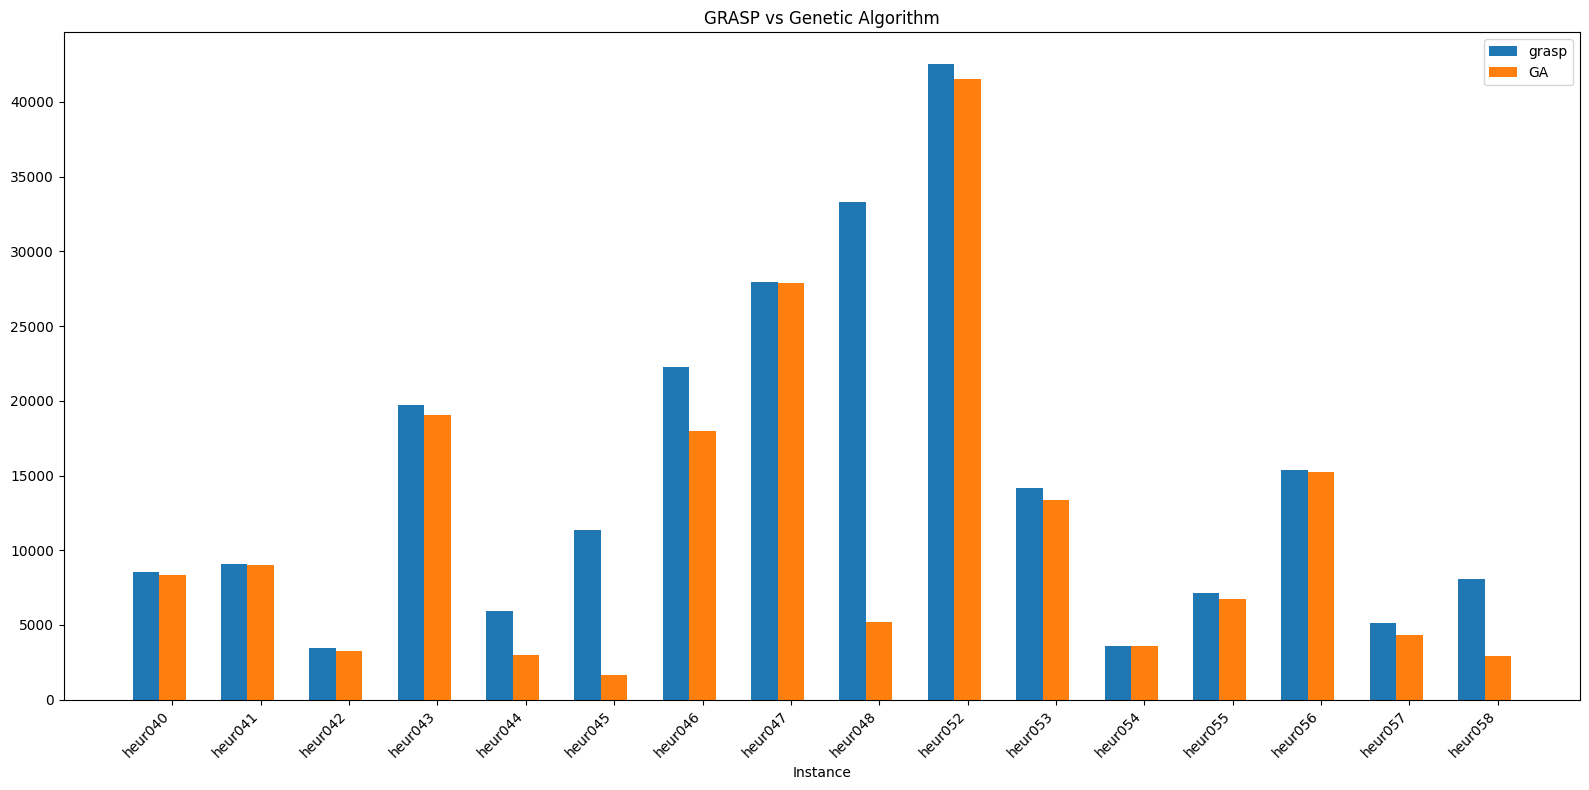
\includegraphics[width=10cm]{graphics/grasp vs ga.png}
\end{figure}

\begin{table}[H]
    \centering
    \begin{tabular}{|l|r|r|r|r|r|r|r|r|r|}
         \hline
         & heur040 & heur041 & heur042 & heur043 & heur044 & heur045 & heur046 & heur047 & heur048 \\
         \hline
         run 1 & 6588 & 7044 & 1497 & 17496 & 3939 & 9508 & 20184 & 25909 & 31551\\
         run 2 & 6589 & 7066 & 1441 & 17523 & 3925 & 9537 & 20138 & 25890 & 30999\\
         run 3 & 6448 & 7109 & 1424 & 17796 & 4001 & 9171 & 20197 & 25917 & 31820\\
         run 4 & 6588 & 7065 & 1448 & 17497 & 3866 & 9164 & 20216 & 25889 & 31486\\
         run 5 & 6612 & 7039 & 1407 & 17632 & 3909 & 9169 & 20401 & 25904 & 31422\\
         run 6 & 6585 & 7200 & 1453 & 17554 & 3915 & 9430 & 20340 & 25982 & 31057\\
         run 7 & 6592 & 7104 & 1443 & 17503 & 3953 & 9208 & 20173 & 25916 & 31209\\
         run 8 & 6588 & 7066 & 1429 & 19617 & 3957 & 9424 & 20340 & 25900 & 30858\\
         run 9 & 6359 & 7040 & 1488 & 17469 & 3896 & 9420 & 20592 & 25956 & 31320\\
        run 10 & 6626 & 7056 & 1492 & 17460 & 3948 & 9317 & 20178 & 25922 & 31280\\
        \hline 
        best   & 6359 & 7039 & 1407 & 17460 & 3866 & 9164 & 20138 & 25889 & 30858\\
        mean   &6557.5&7078.9&1452.2&17727.9&3930.9&9334.8&20275.9&25915.2& 31300.25\\
        \hline
         & heur052 & heur053 & heur054 & heur055 & 'heur056 & heur057 & heur058 & heur059 & heur060 \\
         \hline
         run 1 & 42268 & 12159 & 1560 & 5110 & 13308 & 3104 & 6040 & 13008 & 20399 \\
         run 2 & 40339 & 12159 & 1621 & 5070 & 13297 & 3373 & 6036 & 13395 & 21925 \\
         run 3 & 40230 & 12159 & 1578 & 5115 & 13307 & 3095 & 6016 & 12965 & 20452 \\
         run 4 & 41670 & 12159 & 1597 & 5231 & 13327 & 3076 & 6001 & 12826 & 20836 \\
         run 5 & 40218 & 12159 & 1542 & 5250 & 13440 & 3091 & 6088 & 13064 & 20878 \\
         run 6 & 39825 & 12159 & 1561 & 5095 & 13443 & 3123 & 6048 & 13024 & 20427 \\
         run 7 & 40201 & 12159 & 1576 & 5088 & 13295 & 3070 & 6024 & 12781 & 20549 \\
         run 8 & 40076 & 12159 & 1549 & 5226 & 13443 & 3179 & 5976 & 12856 & 22577 \\
         run 9 & 40156 & 12159 & 1560 & 5056 & 13272 & 3081 & 6233 & 13023 & 20345 \\
        run 10 & 40275 & 12159 & 1589 & 5085 & 13420 & 3041 & 6029 & 13011 & 22045 \\
        \hline
        best   & 39825 & 12159 & 1542 & 5056 & 13272 & 3041 & 5976 & 12781 & 20345\\
        mean   &40525.8&12159.0&1573.3&5132.6&13355.2&3123.3&6049.1&12995.3&21043.3\\
        \hline
    \end{tabular}
    % \caption{Caption}
    \label{tab:my_label}
\end{table}













 
 
 
 
 
 
 
 
 

 
 
 
 
 
 
 




\algdef{SE}[REPEATN]{REPEATN}{END}[1]{\algorithmicrepeat\ #1 \textbf{times}}{\algorithmicend}
\newpage
\section*{Adaptive Large Neighbour Search}
\begin{algorithm}
\caption{ALNS}
given a problem instance $I$ and the hyperparameters $\gamma$ : momentum for $\rho$, $T$ : initial temperature, $\alpha$ : cooling factor.
\begin{algorithmic}
\State $x_0 \gets $ greedy construction 
\State $\rho_d \gets [1, ..., 1]^T$
\State $\rho_r \gets [1, ..., 1]^T$
\While{$T \geq$ stop\_temp}
\REPEATN{\#epochs}
\State $D(\cdot) \gets $pick \textit{destroy} function at random proportional to $\rho_d$
\State $R(\cdot) \gets $pick \textit{repair} function at random proportional to $\rho_r$

\State $x_1 \gets R(D(x_0))$
\State metropolis acceptance of $x_1$ against $x_0$
\State \textbf{record} best solution so far

\END
\State \textbf{update} $\rho_d, \rho_r, T$ 
\EndWhile

\noindent
\Return best recorded solution
\end{algorithmic}
\end{algorithm}

The ALNS we implemented is a class that takes in input a number of hyperparameters and two lists:
\begin{itemize}
    \item \textbf{destroy functions}: functions that take in input a solution $x_0$ and return an altered solution with something changed, note that this solution may not respect the constraints of the problem. 
    \item \textbf{repair functions}: functions that repair a solution which doesn't respect the problem constraint.
\end{itemize}

Then we initialize two lists with ones, representing the initial probabilities of picking one or another destroy/repair functions.

At each loop we're going to extract at random (proportional to $\rho$) a destroy and a repair function, apply them to $x_0$. Then, using the metropolis acceptance, we accept the result with a certain probability, depending on the difference of the objective function values of $x_0$ and $x_1$ and the current temperature $T$.

We're going to run this in a nested loop. The outer loop is going to run until the value of the temperature reaches a value which is small enough: 50 during hyperparameter tuning, 1 when performing the final evaluation.

The inner loop will repeat \#epochs=100 times by default, at the end of which we're going to update $\rho$ with the number of successes of each destroy/repair function, and we're going to update also $T \gets \alpha T$.
$$\rho_d[i] \gets (1-\gamma) \rho_d[i] + \gamma \frac{\#successes(i)}{\#attempts(i)}$$


\subsection*{Destroy Functions}
All our destroy functions modify the partition of the clusters, without considering the damages to the intra-cluster edges:
\begin{itemize}    
    \item \textbf{Merge}: Given 2 random clusters merge them together. This function can be skewed to choose proportionally to the inter-cluster distance;
    \item \textbf{Divide}: given a random cluster divide it in 2 subclusters. This function can be skewed to choose proportionally to intra-cluster distance.
    \item \textbf{SwapNode}: given 2 clusters swap randomly two nodes.
\end{itemize}

\subsection*{Repair Functions}
2 out of 3 of our destroy functions destroy the intracluster edges and the s-plex condition (each node must have at least $|V|-s$ edges with nodes within its plex).
To account for this we have two repair functions that rebuild the edges inside a cluster:
\begin{itemize}
    \item \textbf{Insertion heuristic}: consider a plex with no edges; for each node insert edges (starting from the smallest weight) until it has $|V|-s$ edges.
    \item \textbf{Deletion heuristic} consider a fully connected plex; for each node remove $s$ edges (if possible), starting from those with the highest weight.
\end{itemize}

\subsection*{Hyperparameter tuning}
In this process we have a bunch of hyperparameters:
\begin{itemize}
    \item \textit{stop\_temperature}: temperature at which we stop the execution, it's 50 when doing the hyperparameter search (to speed up the process) and 1 otherwise;
    \item \textit{epochs}: number of repetitions to run in the inner loop, before updating $T$ and $\rho$, by default it's 100;
    \item \textit{initial temperature}: it's the starting temperature $T$;
    \item \textit{alpha}: it's the cooling factor for the temperature;
    \item \textit{gamma}: it's the momentum weight for updating $\rho$.    
\end{itemize}
On the last three parameters we run a grid search on the tuning set to find the best parameters.


\begin{table}[h]
    \centering
    \begin{tabular}{|c|ccc|}
    \hline
        temperature & 100 & 1000 & 10000\\ \hline
        gamma & 0.7 & 0.9 & \\ \hline
        cooling & 0.92 & 0.95 & \\ \hline
    \end{tabular}
    \caption{Test hyperparameters}
    \label{tab:hyperparameter_grid}
\end{table}

We run each of the possible 12 configurations[\ref{tab:hyperparameter_grid}] 10 times on each of the 18 tuning instances, for a total of 2160 runs.
Then we compute the gain for each of the different parameter's configurations as the scaled difference to the mean performance.
$$gain = \frac{f(x_0) - avg(f)}{avg(f)}$$

Now our goal is to find the set of parameters that give us the lowest possible gain (as this is a minimization problem).

\begin{figure}[H]
    \centering
    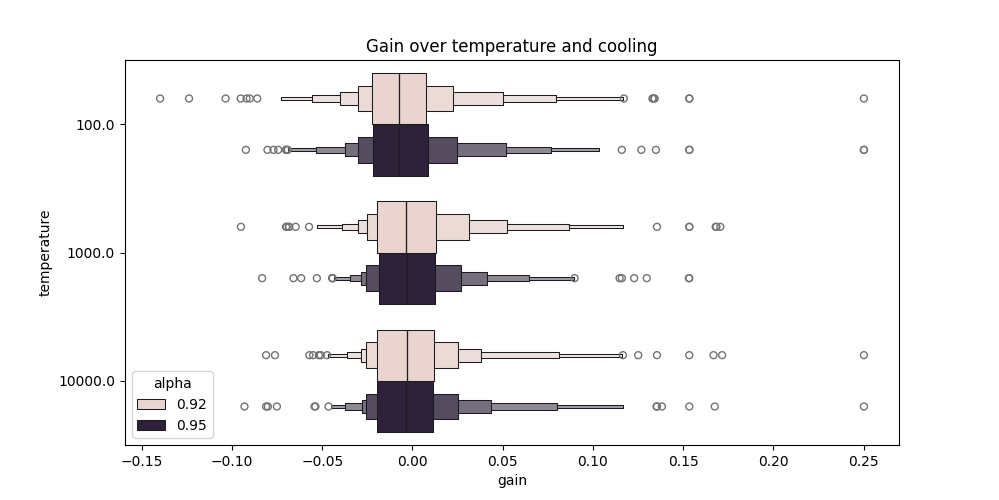
\includegraphics[width=0.8\linewidth]{graphics/Temperature.png}
    \caption{Gain computed for different values of the temperature and cooling factor}
    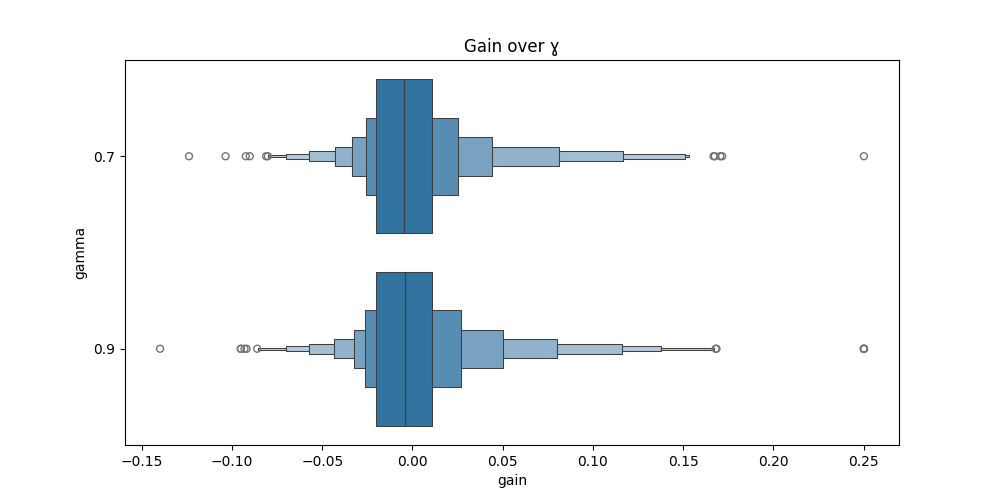
\includegraphics[width=0.8\linewidth]{graphics/gamma.png}
    \caption{Gain computed over different values of gamma}
    \label{fig:enter-label}
\end{figure}

Only by this plots it doesn't seem that the difference is very significant.

We then plot the mean performance of each triplet of parameters:
\begin{figure}[H]
    \centering
    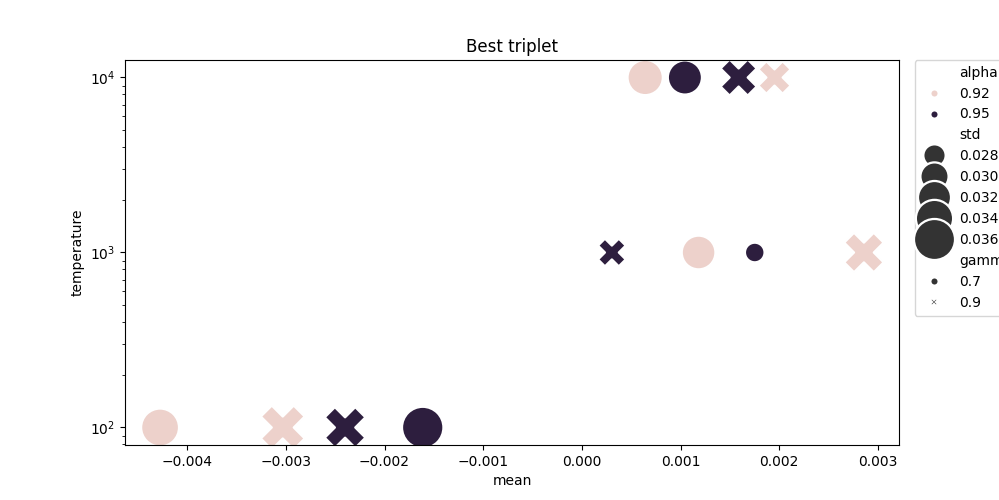
\includegraphics[width=0.9\linewidth]{graphics/best_params.png}
    \caption{Mean objective value for configuration of parameters}
    \label{fig:enter-label}
\end{figure}

We can see that the distances are very small and the standard deviation is very high, but among these the best triplet is:

\begin{table}[h]
    \centering
    \begin{tabular}{|c | c| c|}
        temperature & alpha & gamma\\ \hline
        100 & 0.92 & 0.7\\
    \end{tabular}
    \label{tab:best_params}
\end{table}


\subsection*{Statistical Testing}
\subsubsection*{Frequentist \textit{t}-Test}
We can try to test whether the difference that we see in the plot is significant. The maximum probability that we're willing to consider given the risk of a type I error is 0.05. 
\begin{itemize}
    \item \textbf{H0}: the best performing parameters \ref{tab:best_params} are performing better by chance, their objective values have the same mean as the rest;
    \item \textbf{H1}: the best performing parameters perform better as their mean objective value is lower than objective value than the rest.
\end{itemize}
We perform a one-sided t-test the result of which is:

$$\textbf{p-value} = 0.024674$$

As such we can reject the null hypothesis with a level of significance of 0.05, and assume that the distribution of the gain for the best triplet found is statistically better than the other parameters. As such this configuration will be the one that we'll use for the final submission.

\subsubsection*{Bayesian hypothesis testing}
Since the size of our population is quite small we can try to perform bayesian hypothesis testing, which should be more robust. We test two hypothesis:
\begin{itemize}
    \item \textbf{H0}: the gamma parameter has no influence on the performance;
    \item \textbf{H1}: the gamma parameter is significant.
\end{itemize}
We set as a non-informative prior where $p(H_0) = p(H_1) = 0.5$ as we don't have any information about the distribution of performance of parameters. 
When computing the log-likelihood of the two cases we arrive find out:
$$\textbf{Bayes Factor} = \frac{p(X|H_1)}{p(X|H_0)} = 1.73$$
Which following the Kass and Raftery table\footnote{\href{https://en.wikipedia.org/wiki/Bayes_factor\#Interpretation}{Bayes Factor on Wikipedia}} should be interpreted as "barely any evidence of statistical significance".

As such we can conclude that the gamma parameter isn't very important when it comes to changes in the performance (although admittedly we had the time and resources to test it only on two values). 
\end{document}
